\begin{columns}[t]
	\begin{column}{0.32\textwidth}
		\begin{block}{\large Pose Estimation Evaluation}
			\centering
			\begin{itemize}
				\item Dataset is readily used to compare pose estimation algorithms for this difficult task 
				\item Acceptable accuracy thresholds are at the discretion of the user
				\item May use the metrics provided by the dataset to determine a series of improvements in order to deal with difficulties of the task
			\end{itemize}
				\begin{figure}[h]
					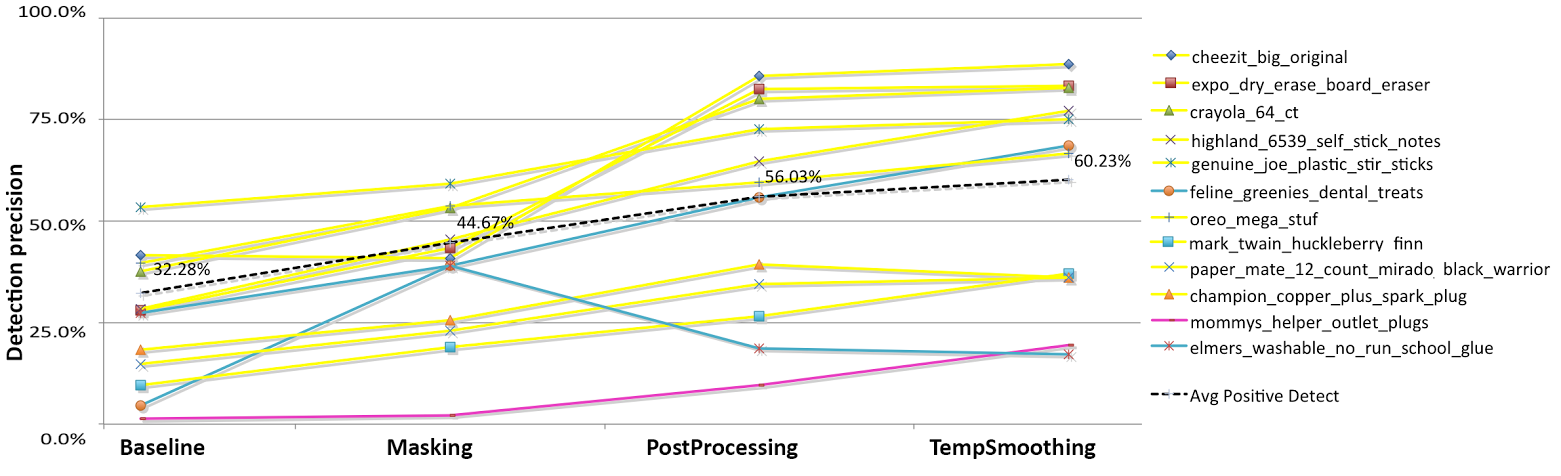
\includegraphics[width = 0.9\textwidth]{results}
					\caption{Evaluation made possible several improvements to an example pose estimation algorithm }
				\end{figure}
				\begin{figure}[h]
					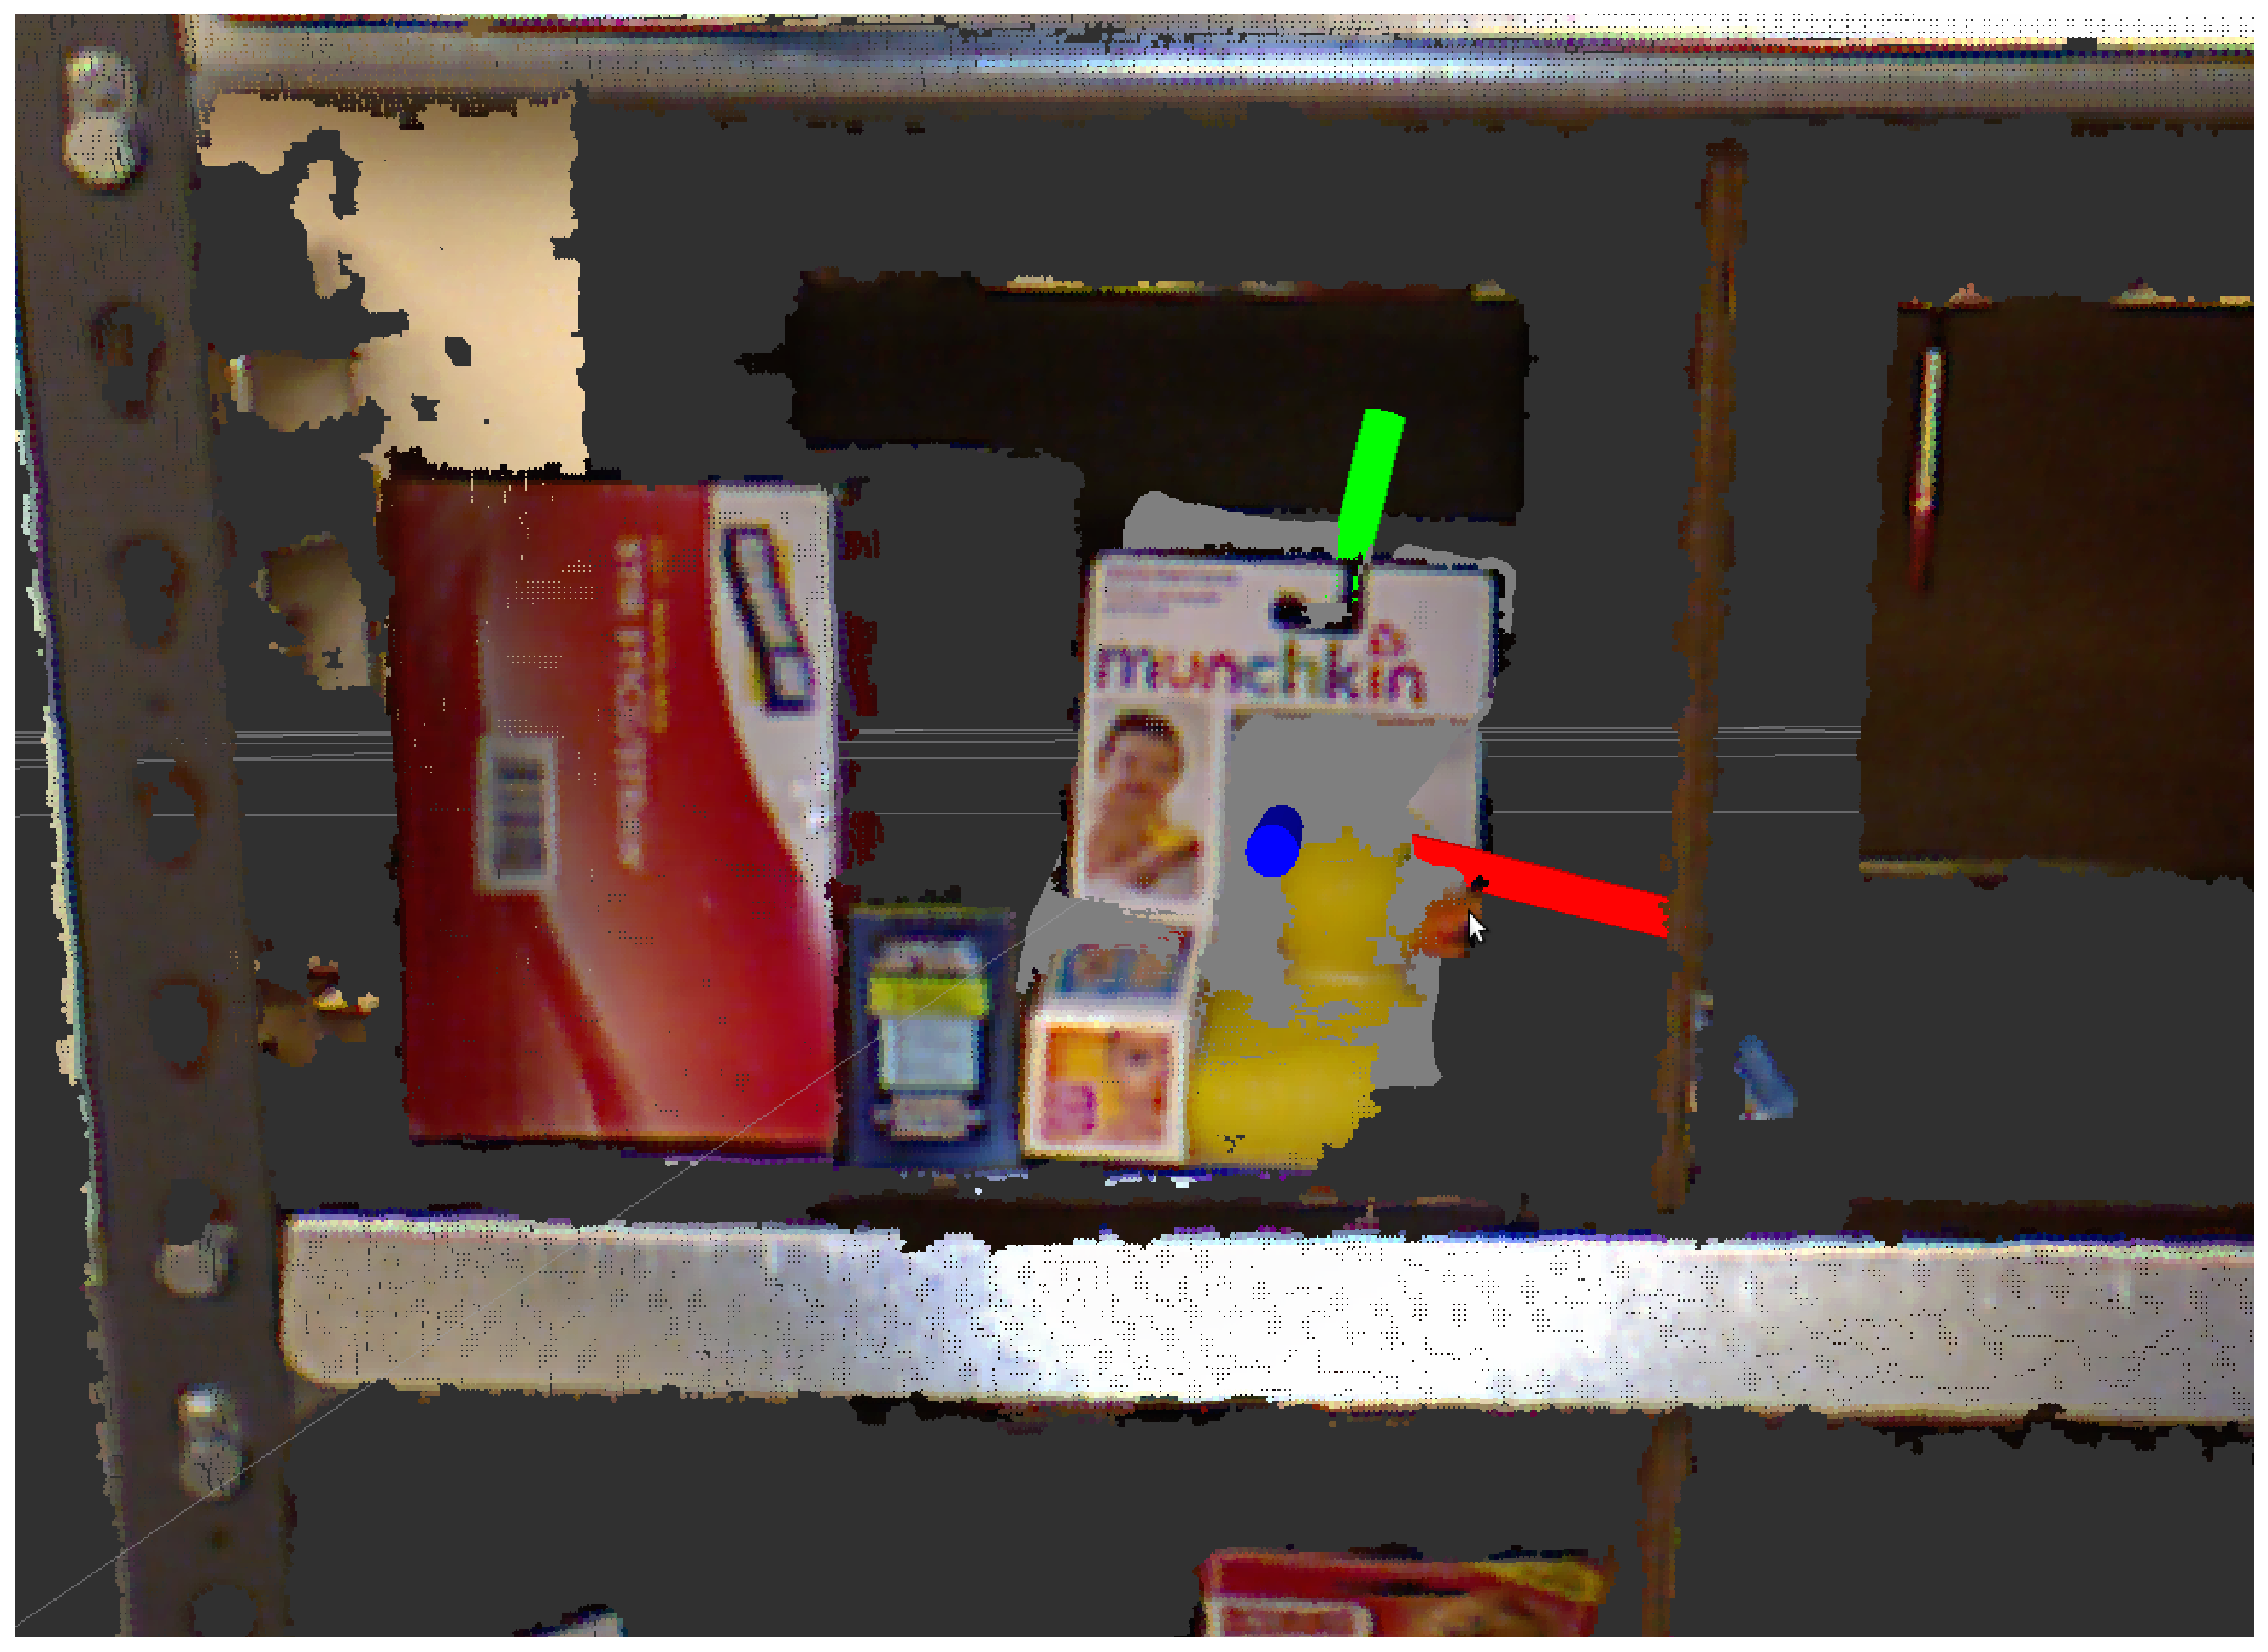
\includegraphics[width = 0.7\textwidth]{munchkin_det}
					\caption {An example detection of the ``duck'' from our dataset}
				\end{figure}
		\end{block}
	\end{column}
	\begin{column}{0.68\textwidth}
		\begin{block}{\large Dataset Comparison}
			\centering
			\vspace{-0.2in}
				\begin{figure}[h]
					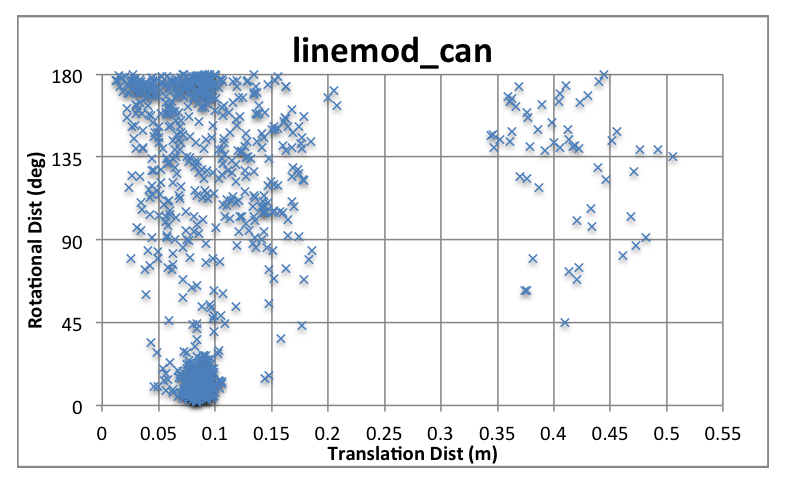
\includegraphics[width = 0.3\textwidth]{linemod_can_results}
					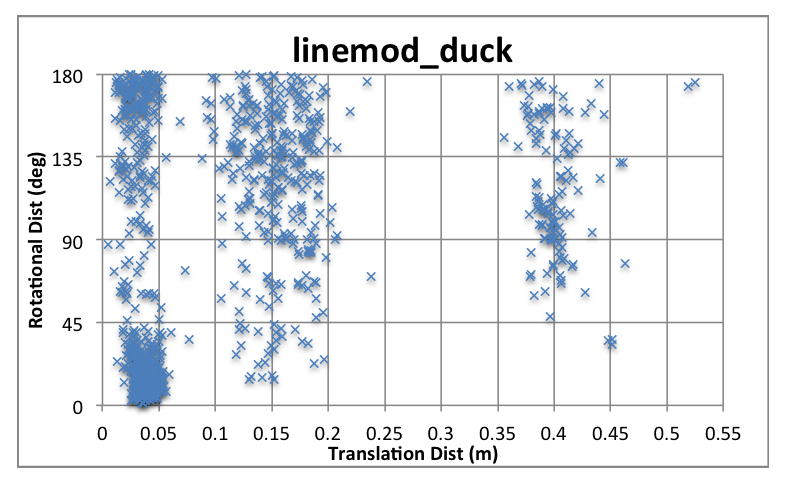
\includegraphics[width = 0.3\textwidth]{linemod_duck_results}
					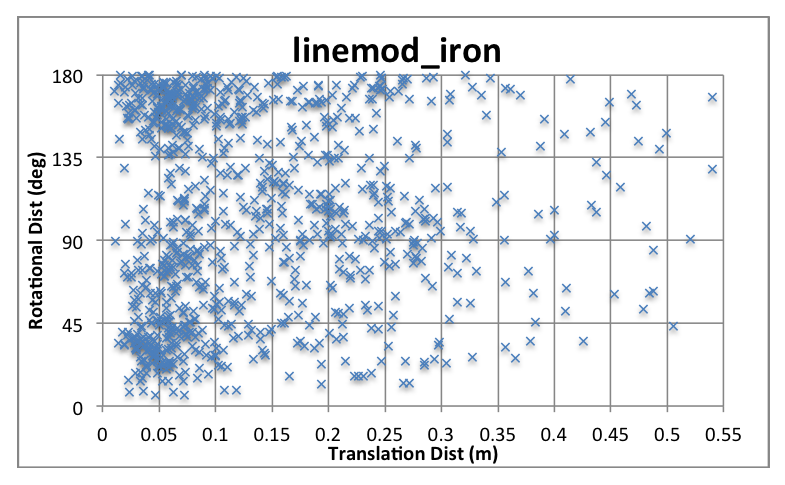
\includegraphics[width = 0.3\textwidth]{linemod_iron_results}
					\vspace{-0.2in}
					\caption{Example objects from LINEMOD dataset evaluated using our example algorithm}
				\end{figure}
			\vspace{-0.2in}
			\begin{itemize}
				\item LINEMOD dataset of 10,000+ RGBD images with ground truth 6D pose
				\item Shows target items on an AR board, in a heavily cluttered environment
				\item Samples generated from a variety of viewpoints around and above the object
				\item Can evaluate rotational, translational accuracy using the provided object models 
			\end{itemize}
				\begin{figure}[h]
					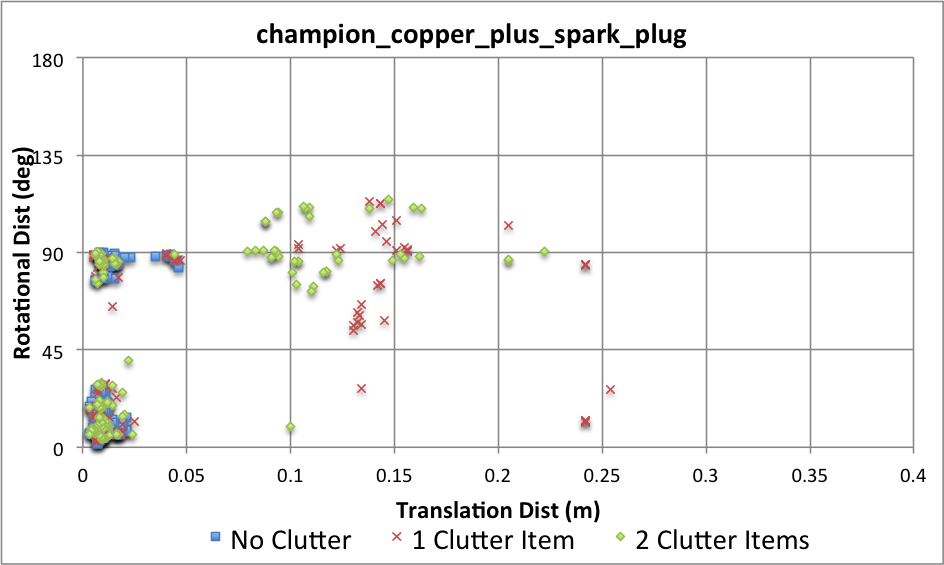
\includegraphics[width = 0.3\textwidth]{scatter_champion}
					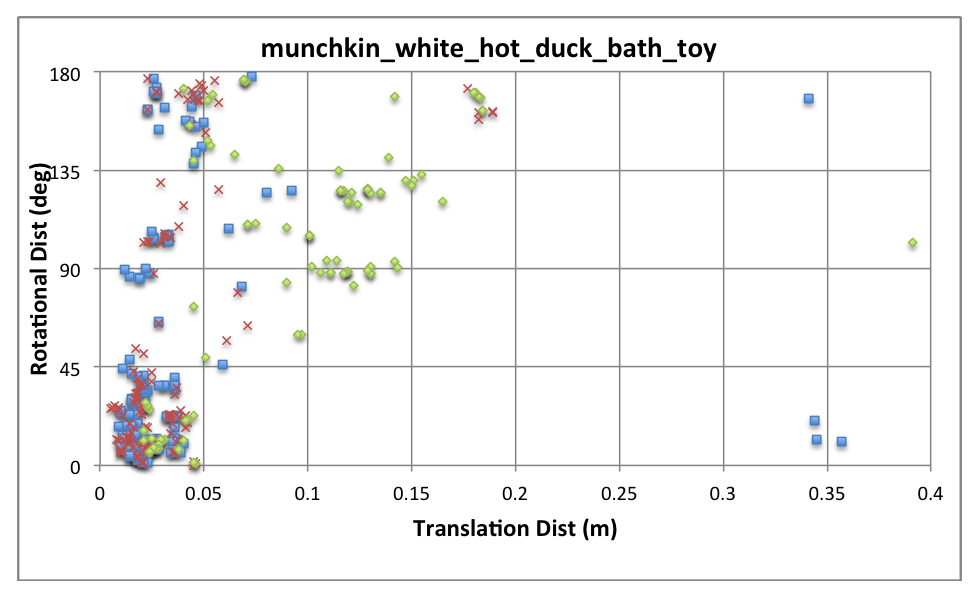
\includegraphics[width = 0.3\textwidth]{scatter_munchkin}
					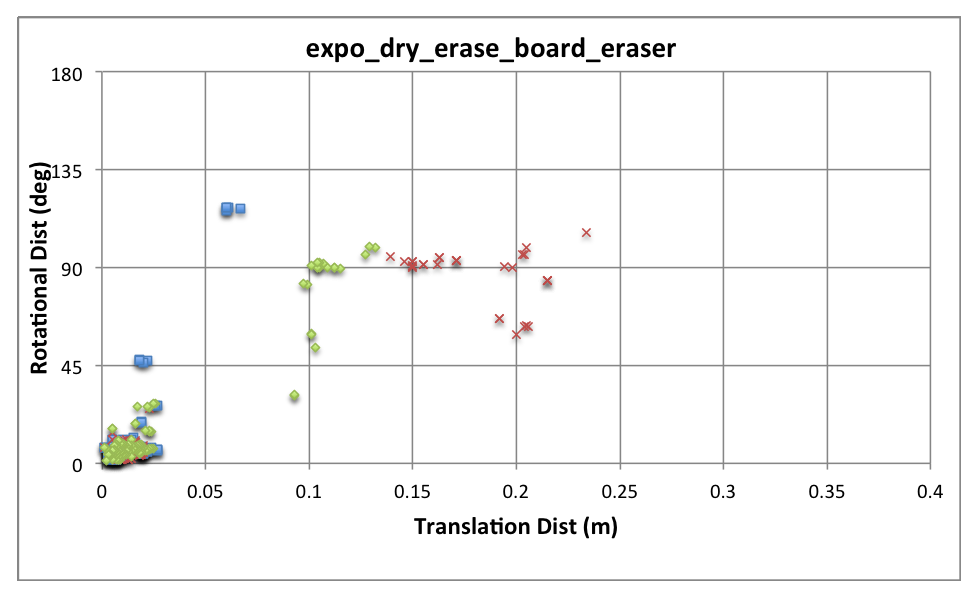
\includegraphics[width = 0.3\textwidth]{scatter_expo}
					\vspace{-0.2in}
					\caption{Objects from our dataset evaluated using the same algorithm; Colors indicate clutter conditions}
				\end{figure}
			\vspace{-0.2in}
			\begin{itemize}
				\item Our similar setup: object models provided, 10,000+ RGBD images
				\item Able to extract effects of immediate clutter on accuracy
				\item Can also determine robustness to noise in the sensor samples
				\item Evaluation with our dataset allows researchers to identify certain weak points in pose estimation algorithms on this difficult task
			\end{itemize}
		\end{block}
	\end{column}
\end{columns}